\documentclass{standalone}
\usepackage[utf8]{inputenc}
\usepackage{amsmath}
\usepackage{tikz}
\usetikzlibrary{calc,positioning}

\begin{document}

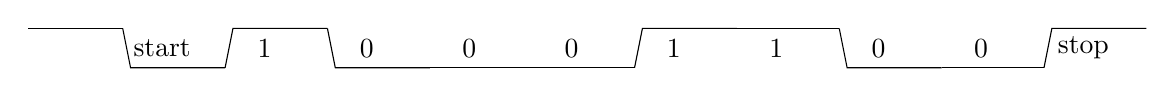
\begin{tikzpicture}
		\coordinate(x) at (0,0);
		\draw
			($(x)+(0.1,0.25)$) -- ++(1.2,0) coordinate (x1)
			($(x)+(1.3,0)$) coordinate (x);
		\draw
			($(x)+(0.5,0)$) node {start}
			(x1) -- ($(x)+(0.1,-0.25)$) -- ++(1.2,0) coordinate (x1)
			($(x)+(1.3,0)$) coordinate (x);
		\foreach \x in {1,0,0,0,1,1,0,0}{
			\draw ($(x)+(0.5,0)$) node {\x}
				\ifnum\x=1
					(x1) -- ($(x)+(0.1,0.25)$)
				\else
					(x1) -- ($(x)+(0.1,-0.25)$)
				\fi
				-- ++(1.2,0) coordinate(x1)
				($(x)+(1.3,0)$) coordinate (x);
			}
		\draw
			($(x)+(0.5,0)$) node {stop}
			(x1) -- ($(x)+(0.1,0.25)$)
			-- ++(1.2,0) coordinate(x1);
\end{tikzpicture}

\end{document}
